\documentclass[tikz]{standalone}

\usepackage{tikz}

\usetikzlibrary{arrows,automata, positioning}




\begin{document}



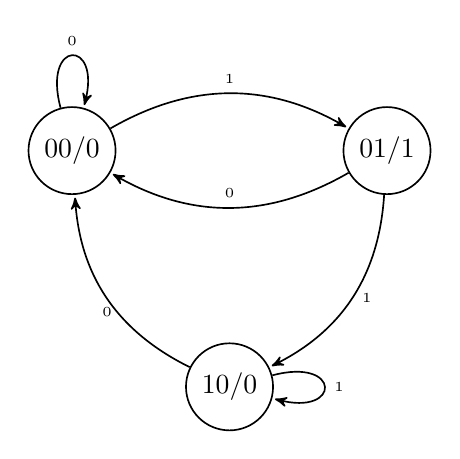
\begin{tikzpicture}[->,>=stealth',shorten >=1pt,auto,node distance=2.8cm,
                    semithick]



\node[state] (1) at(0,0) {$00/0$};
\node[state] (2) at(4,0) {$01/1$};
\node[state] (3) at(2,-3) {$10/0$};


\draw 
(1) edge[loop above] node{\tiny $0$} (1)
(1) edge[above, bend left] node{\tiny $1$} (2)


(2) edge[above, bend left] node{\tiny $0$} (1)
(2) edge[right, bend left] node{\tiny $1$} (3)


(3) edge[loop right] node{\tiny $1$} (3)
(3) edge[below, bend left] node{\tiny $0$} (1)






;\end{tikzpicture}


\end{document}